\section{The Standard Model}
\label{sec:SM}
The current best description we have of the fundamental constituents of our Universe is the Standard Model. It includes the elementary particles and the forces acting between them and can explain all visible matter we have around us (sans gravity). 

The particles in the SM are organized in three generations, as shown in figure \ref{fig:SM}. It consists of two different types of particles, namely fermions and bosons. Fermions are the matter particles, and the bosons carry the forces that act between the fermions and are usually called force particles. 

The elementary particles interact via some force if they carry the \textit{charge} corresponding to the force. Only particles that are electrically charged interact via the electromagnetic force, only particles with (weak) isospin interact via the weak force, and only particles with color charge interact via the strong force.  

\subsection{Standard Model symmetries}
Formally, the three interactions in nature are related to three different symmetry groups. The collective symmetry group of the SM is often represented as

\begin{equation}
    SU(3)_C \otimes SU(2)_L \otimes U(1)_Y, 
    \label{eq:SM_symmetry}
\end{equation}

where $SU(3)_C$ is the symmetry group of the strong force\footnote{More precisely quantum chromodynamics (QCD), which is the quantum field theory of the strong interaction. The C corresponds to color charge being conserved.}, $SU(2)_L$ is the symmetry group of the weak force\footnote{With isospin I as the conserved quantity. The subscript $L$ will be explained later.}, and $U(1)_Y$ is related to the electromagnetic force\footnote{More precisely quantum electrodynamics (QED), which is the quantum field theory of the electromagnetic interaction.}. The $Y$ represents (weak) hypercharge, which is related to electric charge $Q$ and the third component of the isospin $I_3$ through $Y = 2(Q-I_3)$.

Since $SU(2)$ symmetry transformations are defined in terms of 2 x 2 matrices, they need a two-dimensional vector to act upon. Analogously, the $SU(3)$ transformations need to act upon a three-dimensional vector. These vectors are referred to as $SU(2)$ \textit{doublets} and $SU(3)$ \textit{triplets}.


\begin{comment}

They are usually arranged in doublets according to their isospin, that describes their electroweak coupling. Isospin is a quantum number which are related to the strong interaction. It is defined as a vector quantity as

\begin{equation}
    \label{eq:isospin}
    I_{3}={\frac {1}{2}}(n_{u}-n_{d}),
\end{equation}
where $n_u$ is the number of up-type quarks and $n_d$ is the number of down-type quarks. 
\end{comment}

%In the SM model we look at left-handed particles\footnote{}, which means that these are arranged in doublets according to their isospin


%The isospin is connected to flavor symmetry which you can easily see in baryons (qqq) and mesons ($q\Bar{q}$), where we also can get isospin singlets. 

\begin{figure}[H]
    \centering
    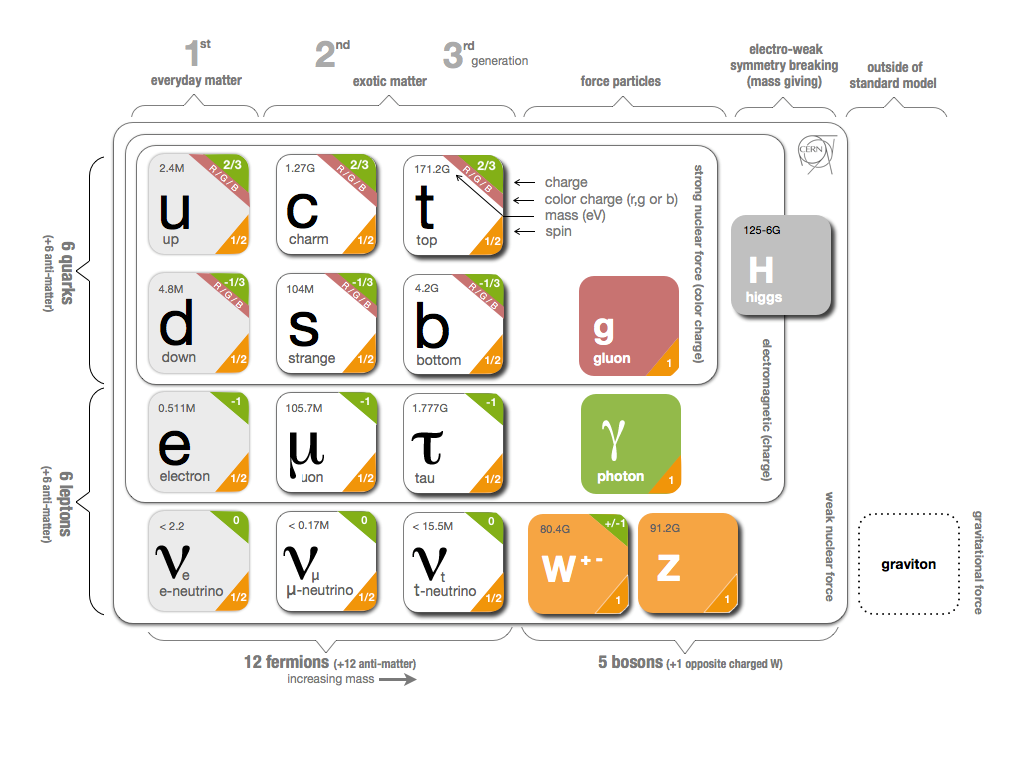
\includegraphics[width=\textwidth]{Figures/FromOnline/SM.png}
    \caption{An overview of the particles in the Standard Model \cite{SMpicture}.}
    \label{fig:SM}
\end{figure}

\subsection{Fermions}
If we look at figure \ref{fig:SM}, we can see that there are 12 different fermions split up in two groups called quarks and leptons, which again are split up into three generations. The lightest quarks and leptons are in the first generation, and the most massive quarks are in the third generation. All of the fermions are $\frac{1}{2}$-spin\footnote{Spin is an intrinsic property of all fundamental particles, which can be seen as some kind of internal angular momentum.} particles and differ by mass and electric charge. They also obey the Pauli exclusion principle, which means that only one fermion can occupy a given quantum state for any given set of quantum numbers. 

Further, it is well known that parity\footnote{Parity is spatial inversion.} is violated for the weak interaction. This can be explained by introducing \textit{chirality} which is, using projection operators $P_L$ and $P_R$, defined as 

\begin{equation}
    \label{eq:chirality}
    P_L = \frac{1}{2}(1-\gamma^5) \text{  and  } P_R = \frac{1}{2}(1 + \gamma^5).
\end{equation}

From this, fermions can be separated into a left-chiral and right-chiral part, where only the left-chiral part of a fermion is charged under the weak force (corresponding to the $L$ in equation \ref{eq:SM_symmetry}). It is thus the left-chiral parts of fermions that are put into $SU(2)$ doublets\footnote{The right-chiral parts are said to be $SU(2)$ singlets, meaning that they are not affected bt the weak force.}.

\subsubsection{Quarks}
We have six different quarks in the SM, and they differ by mainly mass, but also charge (both electrical and color charge). All up-type quarks, which are the three quarks in the first row in figure \ref{fig:SM}, have electric charge +2/3, and all down-type quarks, which is in the second row in figure \ref{fig:SM}, have electric charge -1/3. Since they carry a non-zero electric charge, they interact via the electromagnetic force. 


They can also interact with the weak force, which allows all possible combinations of quarks that differ by one unit of charge in doublets: 

\begin{align}
    \binom{u_L}{d_L} \text{,  } \binom{u_L}{s_L} \text{,  } \binom{u_L}{b_L} \text{,  } \binom{c_L}{d_L} \text{,  } \binom{c_L}{s_L} \text{,  } \binom{c_L}{b_L} \text{,  } \binom{t_L}{d_L} \text{,  } \binom{t_L}{s_L} \text{,  } \binom{t_L}{b_L}.
\end{align}

The two quarks in the first generation, namely up (u) and down (d), are the constituents of the protons (uud) and neutrons (ddu) - which then combine in various ways to form atomic nuclei. The second and third generation of quarks (charm, strange, top and bottom) are more massive than the quarks in the first generation. Since the quarks in the second and third generations are more massive, they need more energy to exist and will therefore decay to lighter particles very fast. 

Quarks also carry color charge, which allows them to couple to different gluons through the strong interaction in quantum chromodynamics (QCD). Quarks are the only known particles that interact with all the fundamental forces. 

Further, quarks can mix between generations, as described by the CKM matrix \cite{thomson}.

%Note that the quarks can be described by either mass eigenstates corresponding to the free-propagating Hamiltonian, or weak eigenstates corresponding to the way they interact under the weak interaction. Those sets of eigenstates do not coincide but are instead related to each other by the CKM matrix \cite{thomson}. 




\subsubsection{Leptons}
Leptons are the other six fermions of the SM. Like quarks, they come in three generations and can be arranged in doublets:

\begin{align}
    \binom{\nu_{eL}}{e_L} \text{,  } \binom{\nu_{\mu L}}{\mu_L} \text{,  } \binom{\nu_{\tau L}}{\tau_L}.
\end{align}

They also differ by mass and electric charge where the lower component has charge -1, and the upper has no charge. Because of that, neutrinos only interact with weak bosons, while for the electron, muon and, tau, electromagnetic interactions are also possible. In the SM the neutrinos are assumed to be massless, but we know from neutrino oscillation experiments that this is not true. However, exactly how the neutrinos acquire mass and why they are so much lighter than all of the other particles in the SM is not yet understood. 

Analogously to quarks, fermion mass and weak eigenstates do not coincide and they are related by the PMNS matrix \cite{thomson}. This phenomenon provides an explanation of neutrino oscillations, where after some distance from the interaction point we measure a different neutrino flavor. 


\subsection{Bosons}
On the right-hand side of figure \ref{fig:SM}, the integer spin particles (spin-0, 1, 2) known as bosons are shown. Bosons follow Bose-Einstein statistics and contain the force carriers for the electromagnetic force, the weak force, and the strong force. If gravity was included in the Standard Model, it would have been through an extra boson, the graviton ($G$). The graviton is believed to have spin-2, which together with the Higgs boson that has spin-0 is the only two bosons that differs in spin from the force carriers with spin-1. Higgs is also so far the only scalar particle detected.



\subsubsection{The strong nuclear force}
The strong nuclear force is mediated by the gluon (g) and couples to the three color charges r (red), g (green), b (blue). Moreover, as suggested by the name, it has a very strong coupling to quarks, and it is responsible for the fact that quarks do not appear as free, unbounded particles. The gluon is massless, and unlike the other forces, it can couple with itself, as you can see in the Feynman diagrams\footnote{Feynman diagrams are a way to graphically represent interactions between particles.} in figure\ref{fig:gluon_self_int}.

\begin{figure}[H]
    \centering
    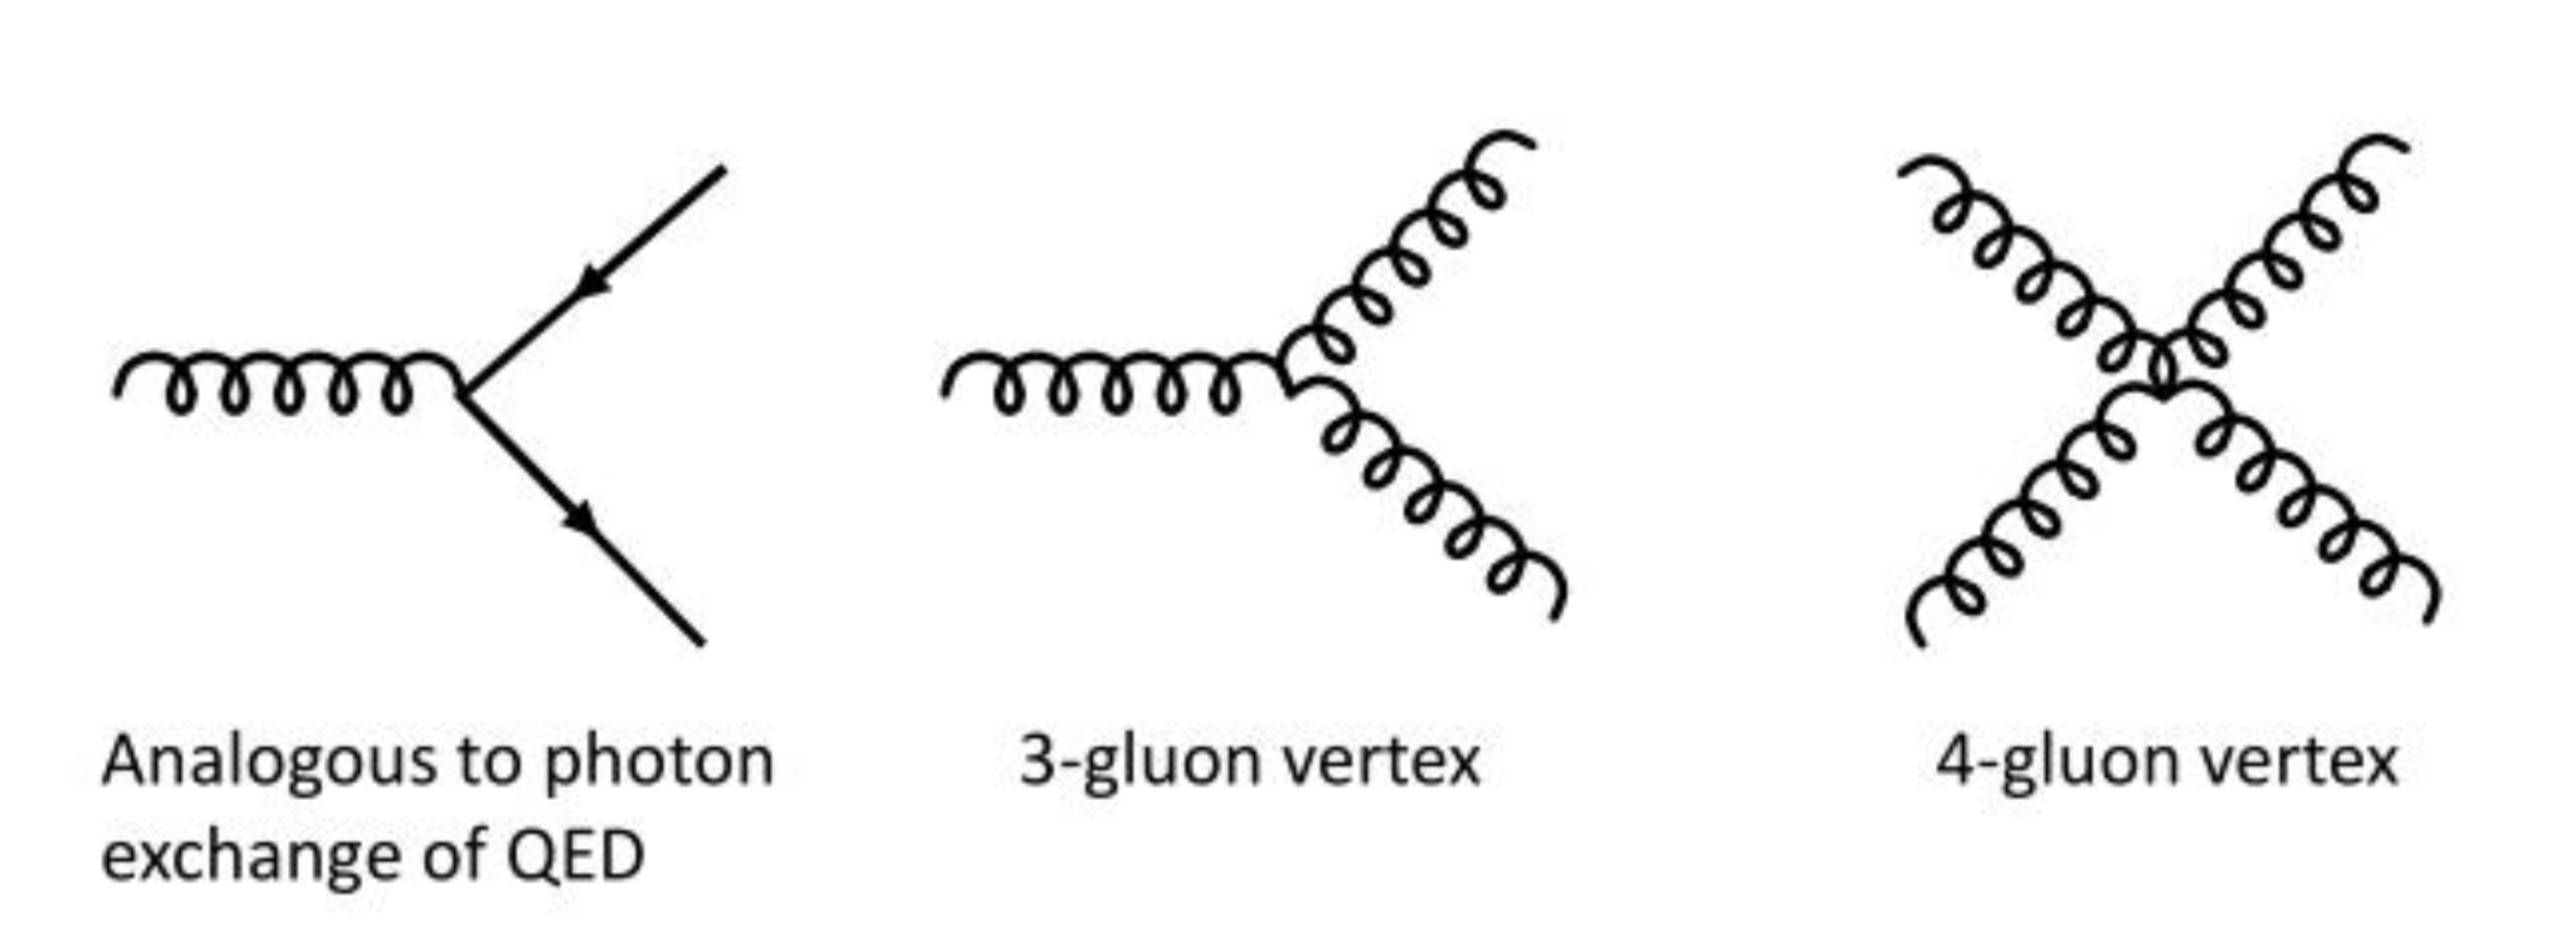
\includegraphics[width = \textwidth]{Figures/FeynmanDiagrams/gluon.pdf}
    \caption{Feynman diagrams for the strong force vertices, where the curly lines represent the gluons \cite{STRONGforce}.}
    \label{fig:gluon_self_int}
\end{figure}

\subsubsection{The electromagnetic force}
The electromagnetic force is mediated by the photon ($\gamma$) and couples to all fermions with electric charge, namely all the quarks and leptons except for the neutrinos. As for the gluon, it has no mass, but since it is electrical neutral it cannot couple to itself. 

\begin{figure}[H]
    \centering
    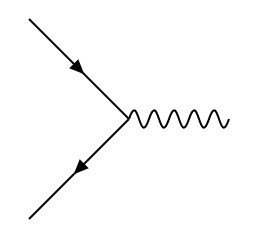
\includegraphics[width = 0.4\textwidth]{Figures/FeynmanDiagrams/photon.png}
    \caption{A Feynman diagram of the electromagnetic vertex, where the wiggly line represent the photon \cite{EMforce}.}
    \label{fig:my_label}
\end{figure}

\subsubsection{The weak nuclear forces}
The weak nuclear forces are mediated by the $W^\pm$-bosons and the $Z^0$-boson. They couple to all particles in the SM, and unlike the other force particles, they have mass. This feature is explained in the GWS model \cite{Xin2007GlashowWeinbergSalamMA} through a spontaneous symmetry breaking due to a non-zero vacuum expectation value that adds an extra degree of freedom to otherwise massless force carriers. It is also the only interaction known to allow flavor change, which means that e.g., an up quark can become a down quark or a muon become an electron as shown in figure\ref{fig:weak_force_FD}. 

\begin{figure}[H]
    \centering
    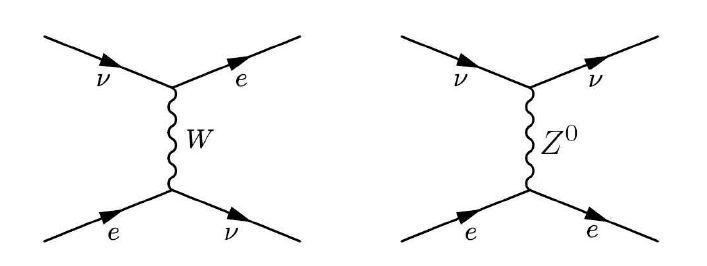
\includegraphics[width = 0.8\textwidth]{Figures/FeynmanDiagrams/weak.png}
    \caption{Feynman diagrams of the weak force vertices \cite{WEAKforce}.}
    \label{fig:weak_force_FD}
\end{figure}

Note that the physical bosons $\gamma, Z^0, W^\pm$ are not the mediators associated to the single symmetry groups, but are instead a linear combination of those states explained by the spontaneous symmetry breaking leading to the electroweak theory. 

\subsubsection{The Higgs boson}

The final piece, the Higgs boson (H), that was missing in the SM was discovered in 2012 at CERN \cite{Higgs_ATLAS, Higgs_CMS}. The discovery gives increased credence to the SM and explains why the weak force carriers, $Z^0$ and $ W^\pm $, have mass. The fermion masses can also be explained by couplings to the Higgs boson. 

